\documentclass{beamer}

\usepackage{amsmath,amssymb}
\usepackage[most]{tcolorbox}
\usepackage{tikz}
\usetikzlibrary{arrows.meta, positioning, shapes.geometric, fit}

% ---------- BASE THEME (kept plain, no navigation-bar theme) ----------
\usetheme{default}
\usefonttheme{professionalfonts}
\setbeamertemplate{navigation symbols}{}
\setbeamercolor{page number in head/foot}{fg=black!50}
\setbeamertemplate{footline}{%
  \hfill\usebeamercolor[fg]{page number in head/foot}%
  \small\insertframenumber{}/\inserttotalframenumber\kern1em\vskip4pt%
}

% ---------- COLORS ----------
\definecolor{lavenderbg}{RGB}{213, 212, 241}
\definecolor{navy}{RGB}{35, 35, 120}
\setbeamercolor{structure}{fg=navy}
\setbeamercolor{frametitle}{bg=lavenderbg, fg=black}
\setbeamercolor{title}{fg=black}
\setbeamerfont{frametitle}{series=\bfseries, size=\Large}

% ---------- FULL-WIDTH FRAMETITLE BAR ----------
\setbeamertemplate{frametitle}{
  \nointerlineskip
  \begin{beamercolorbox}[wd=\paperwidth,ht=4.2ex,dp=1.6ex,leftskip=0.4cm]{frametitle}
    \usebeamerfont{frametitle}\insertframetitle
  \end{beamercolorbox}
}

% ---------- SPACING ----------
\setbeamersize{text margin left=8mm, text margin right=8mm}
\setlength{\parskip}{4pt}

\begin{document}

% ================= Slide 1 : Title =================
\begin{frame}[plain]
\vspace{0.4cm}
\begin{center}
\begin{tcolorbox}[
  enhanced, colback=lavenderbg, colframe=lavenderbg,
  arc=4mm, boxrule=0pt, width=0.94\textwidth,
  halign=center, valign=center,
  drop shadow
]
{\Large\textbf{Customer Churn Prediction \& Lifetime Value (LTV) Engine}}\\[10pt]
{\large AI \& Data Engineering Project Milestone}
\end{tcolorbox}
\end{center}

\vspace{1.3cm}
\begin{center}
{\Large Gopi M -- CB.PS.I5DAS22114}\\[10pt]
{\large Adventure Technology Solutions}\\[10pt]
{\large \today}
\end{center}
\end{frame}

% ================= Slide 2 : Introduction =================
\begin{frame}{Introduction}

\textbf{Objective} \\
Design and implement an end-to-end predictive analytics engine that flags telecom subscriber attrition (churn) and forecasts long-term revenue (Lifetime Value - LTV).

\vspace{2pt}
\textbf{Key Highlights}
\begin{itemize}
    \item \textbf{Dual-Target ML}: Predicts binary churn probability and LTV concurrently for incoming user profiles.
    \item \textbf{Stacked Inference}: Predicts churn status first, then injects it as a feature to condition the LTV regression.
    \item \textbf{Automated Pipeline}: Moves data from PostgreSQL tables to a FastAPI serving backend.
    \item \textbf{BI Visualization}: Integrates Metabase dashboards to display real-time retention and revenue metrics.
\end{itemize}

\end{frame}

% ================= Slide 3 : Problem Statement =================
\begin{frame}{Problem Statement}

Telecom operators face high customer acquisition costs (CAC); retaining an existing subscriber is up to 5x cheaper than acquiring a new one.

\vspace{2pt}
\textbf{Key Challenges}
\begin{itemize}
    \item \textbf{Imbalanced Dataset}: Telecom databases exhibit high class skew (e.g.\ 73.46\% retained vs.\ 26.54\% churned out of 7,043 instances).
    \item \textbf{Database Casing Conflicts}: Case-sensitive SQL headers created by default data frames block visual queries in Metabase.
    \item \textbf{Data Leakage risk}: Naive preprocessing outside pipeline folds invalidates validation boundaries.
    \item \textbf{Static Value Tracking}: Simple LTV estimates fail if they do not account for active churn probabilities.
\end{itemize}

\end{frame}

% ================= Slide 4 : Architecture (Flow Diagram) =================
\begin{frame}{Architecture Overview}
\centering
\resizebox{\textwidth}{!}{%
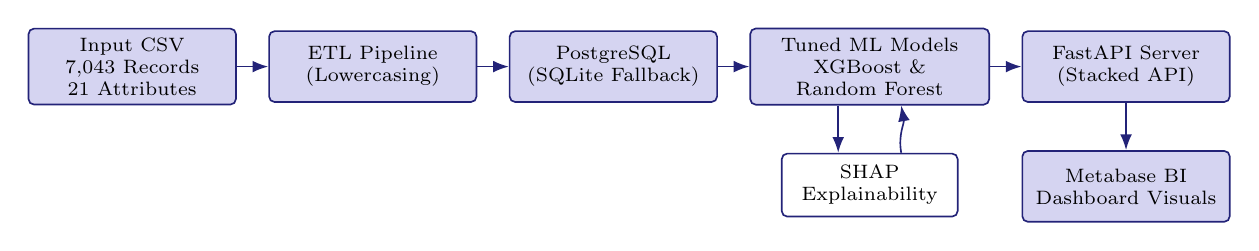
\begin{tikzpicture}[
  font=\scriptsize,
  box/.style={rectangle, rounded corners=2pt, draw=navy, fill=lavenderbg,
    text width=2.4cm, align=center, minimum height=0.9cm, line width=0.6pt},
  loopbox/.style={rectangle, rounded corners=2pt, draw=navy, fill=white,
    text width=2.0cm, align=center, minimum height=0.8cm, line width=0.6pt},
  arr/.style={-{Latex[length=2mm]}, navy, line width=0.6pt}
]
 
\node[box] (input) {Input CSV\\7,043 Records\\21 Attributes};
\node[box, right=0.4cm of input] (etl) {ETL Pipeline\\(Lowercasing)};
\node[box, right=0.4cm of etl] (db) {PostgreSQL\\(SQLite Fallback)};
\node[box, right=0.4cm of db, text width=2.8cm] (ml) {Tuned ML Models\\XGBoost \& Random Forest};
\node[box, right=0.4cm of ml] (api) {FastAPI Server\\(Stacked API)};
 
\node[loopbox, below=0.6cm of ml] (shap) {SHAP\\Explainability};
 
\node[box, below=0.6cm of api, text width=2.4cm] (meta) {Metabase BI\\Dashboard Visuals};
 
\draw[arr] (input) -- (etl);
\draw[arr] (etl) -- (db);
\draw[arr] (db) -- (ml);
\draw[arr] (ml) -- (api);
\draw[arr] (api) -- (meta);
 
\draw[arr] ([xshift=-4mm]ml.south) -- ([xshift=-4mm]shap.north);
\draw[arr] ([xshift=4mm]shap.north) to[out=100,in=-80] ([xshift=4mm]ml.south);
 
\end{tikzpicture}%
}
 
\vspace{6pt}
\footnotesize The ETL script processes and lowercases raw billing headers. Validated FastAPI endpoints draw records from database engines to return real-time estimations.
\end{frame}

% ================= Slide 5 : Outcomes & Technical Results =================
\begin{frame}{Implementation Outcomes \& Key Results}

\textbf{Technical Outcomes}
\begin{itemize}
    \item \textbf{Data Imbalance Fix}: Used XGBoost cost-sensitive parameter `scale\_pos\_weight = 2.7686` to handle class skew.
    \item \textbf{Uptime Fallback}: Session generator auto-redirects to SQLite when local PostgreSQL engines time out.
    \item \textbf{Explainable AI}: Integrated SHAP to explain billing and tenure features.
\end{itemize}

\vspace{4pt}
\textbf{Key Performance Results}
\begin{itemize}
    \item \textbf{Churn Classification (XGBoost)}: Captured **81.28\%** of true churners (**F1-Score: 0.6307**, **Recall: 81.28\%**).
    \item \textbf{LTV Estimation (Random Forest Regressor)}: Reached **$R^2$ of 0.9992** and a Mean Absolute Error of only **\$40.79**.
\end{itemize}

\end{frame}

% ================= Slide 6 : Thank You =================
\begin{frame}[plain]
\vspace{2cm}
\begin{center}
\begin{tcolorbox}[
  enhanced, colback=lavenderbg, colframe=lavenderbg,
  arc=4mm, boxrule=0pt, width=0.7\textwidth,
  halign=center, valign=center,
  drop shadow
]
{\Large\textbf{Thank You}}
\end{tcolorbox}
\end{center}

\end{frame}

\end{document}
